\FloatBarrier
\subsection{Run-by-run check}

\begin{figure}[ht]
    \begin{subfigure}{.49\textwidth}
        \centering
        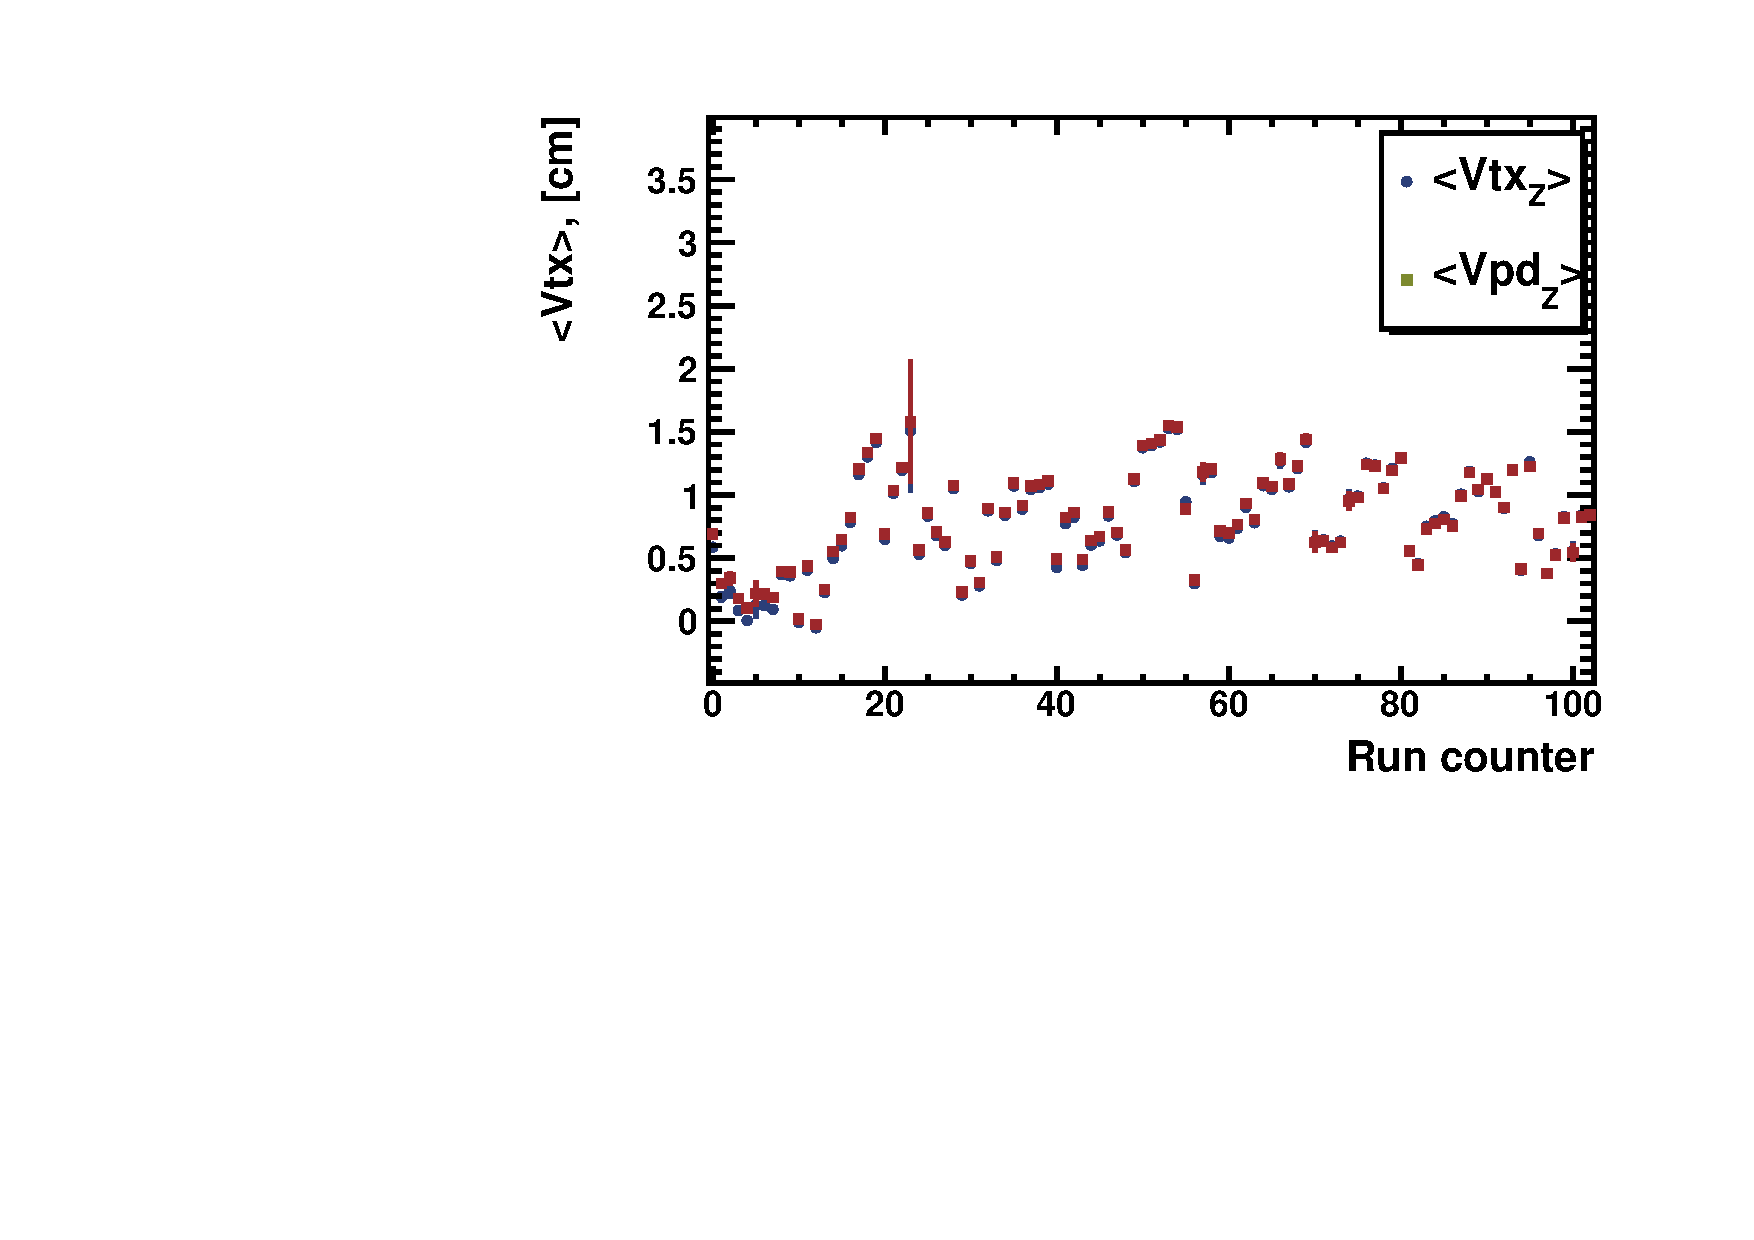
\includegraphics[width=1.\linewidth]{Figures/VtxZVsRun.pdf}
        %\caption{a}
    \end{subfigure}
    \begin{subfigure}{.49\textwidth}
        \centering
        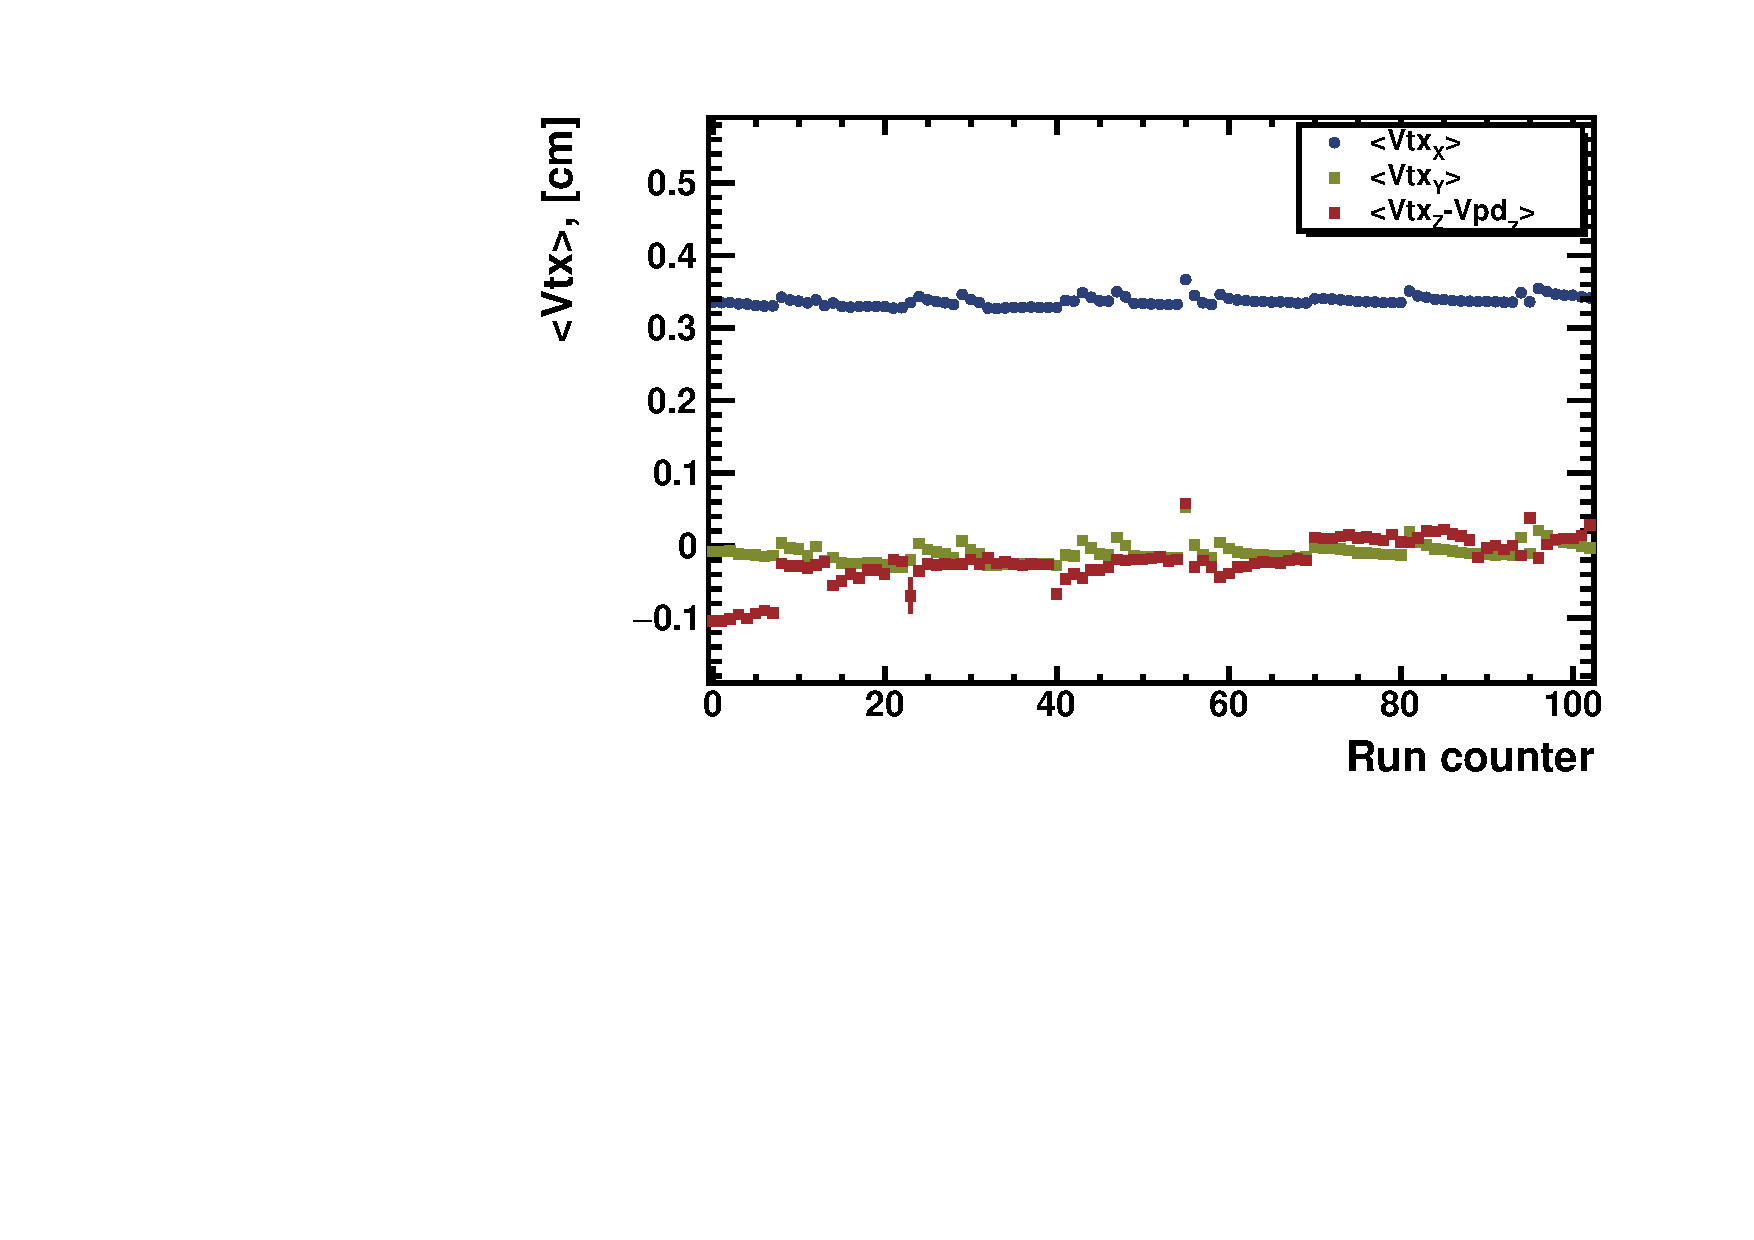
\includegraphics[width=1.\linewidth]{Figures/VtxXYVsRun.pdf}
        %\caption{b}
    \end{subfigure}
    \label{fig:VtxVsRun}
    \caption{Distributions of the $Vtx_Z$, $Vpd_Z$ (left) and $Vpd_X$, $Vpd_Y$, $Vtx_Z - Vpd_Z$ (right) as a function of run.}
\end{figure}

\begin{figure}[ht]
    \begin{subfigure}{.49\textwidth}
        \centering
        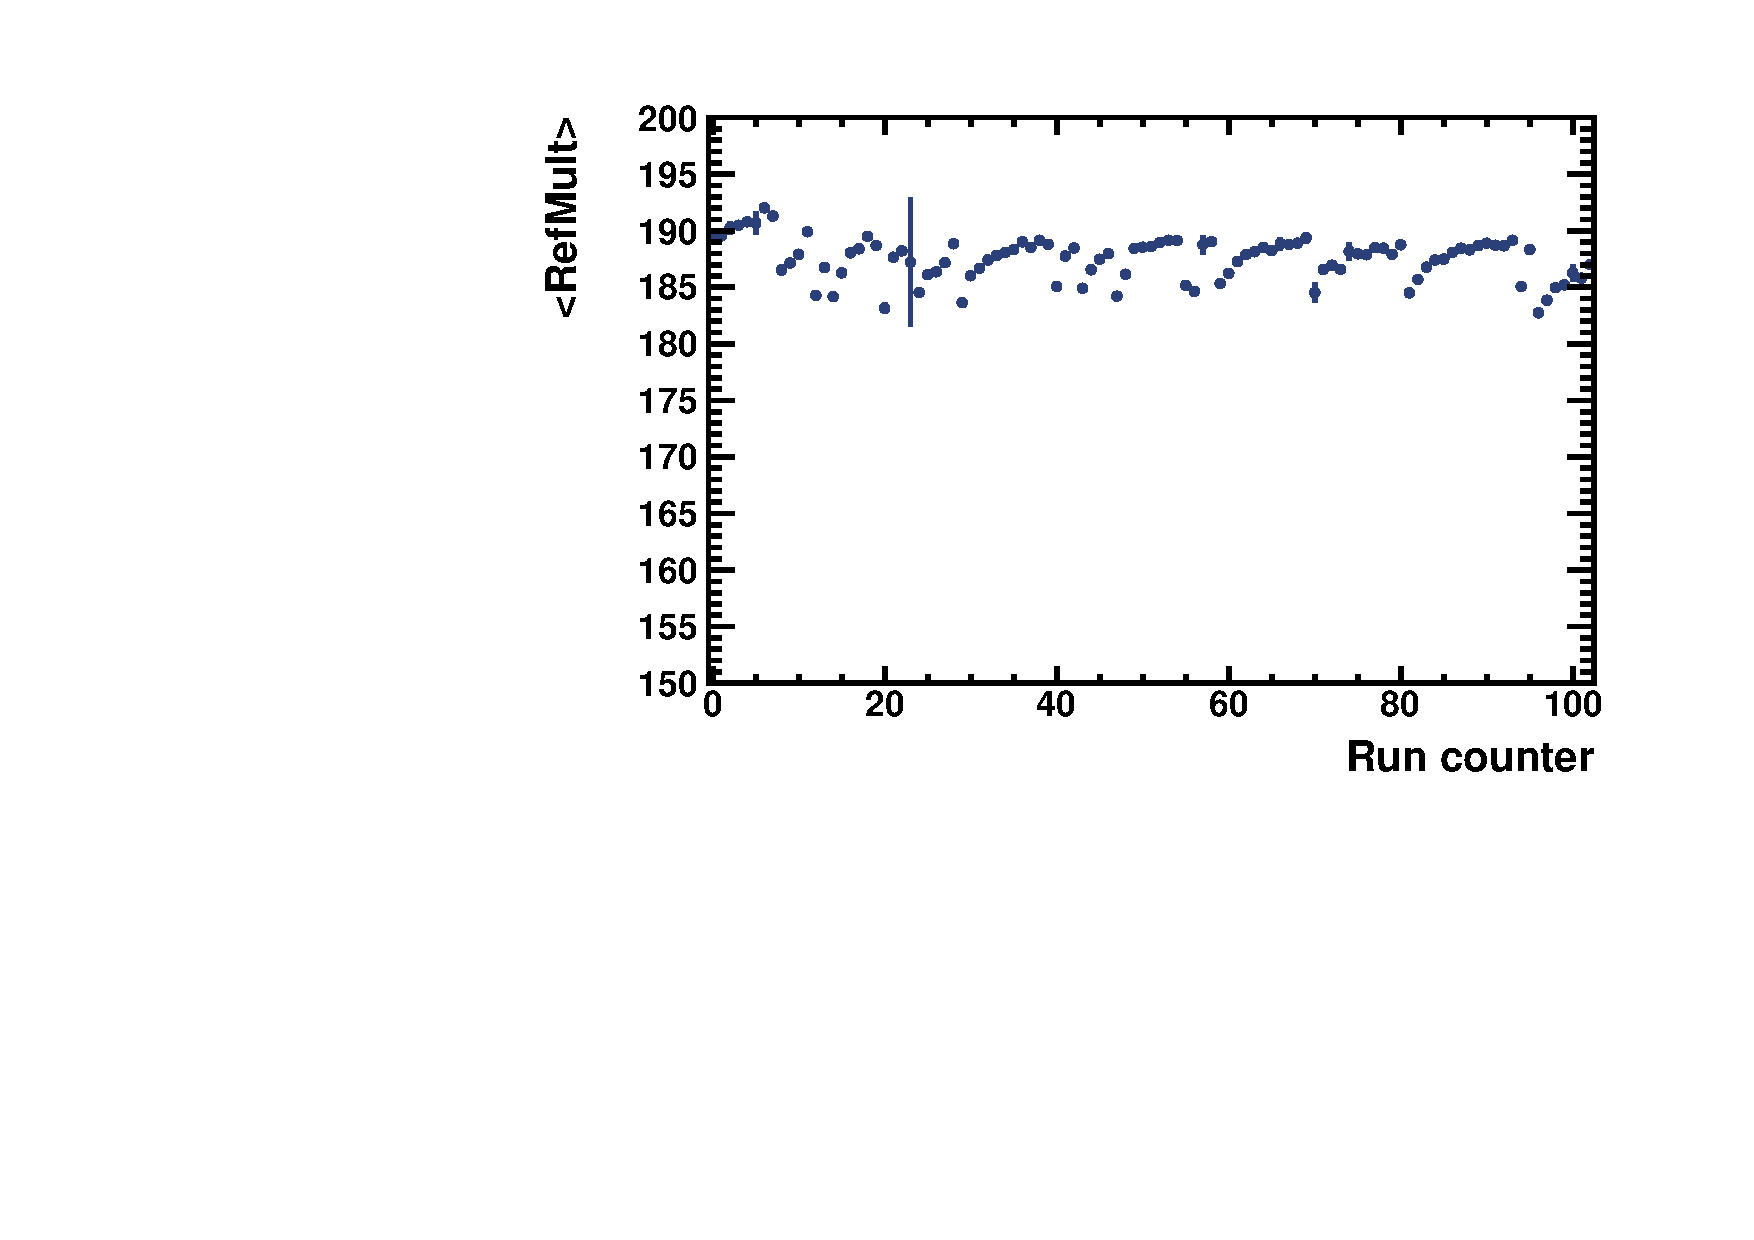
\includegraphics[width=1.\linewidth]{Figures/RefMultVsRun.pdf}
        %\caption{a}
    \end{subfigure}
    \begin{subfigure}{.49\textwidth}
        \centering
        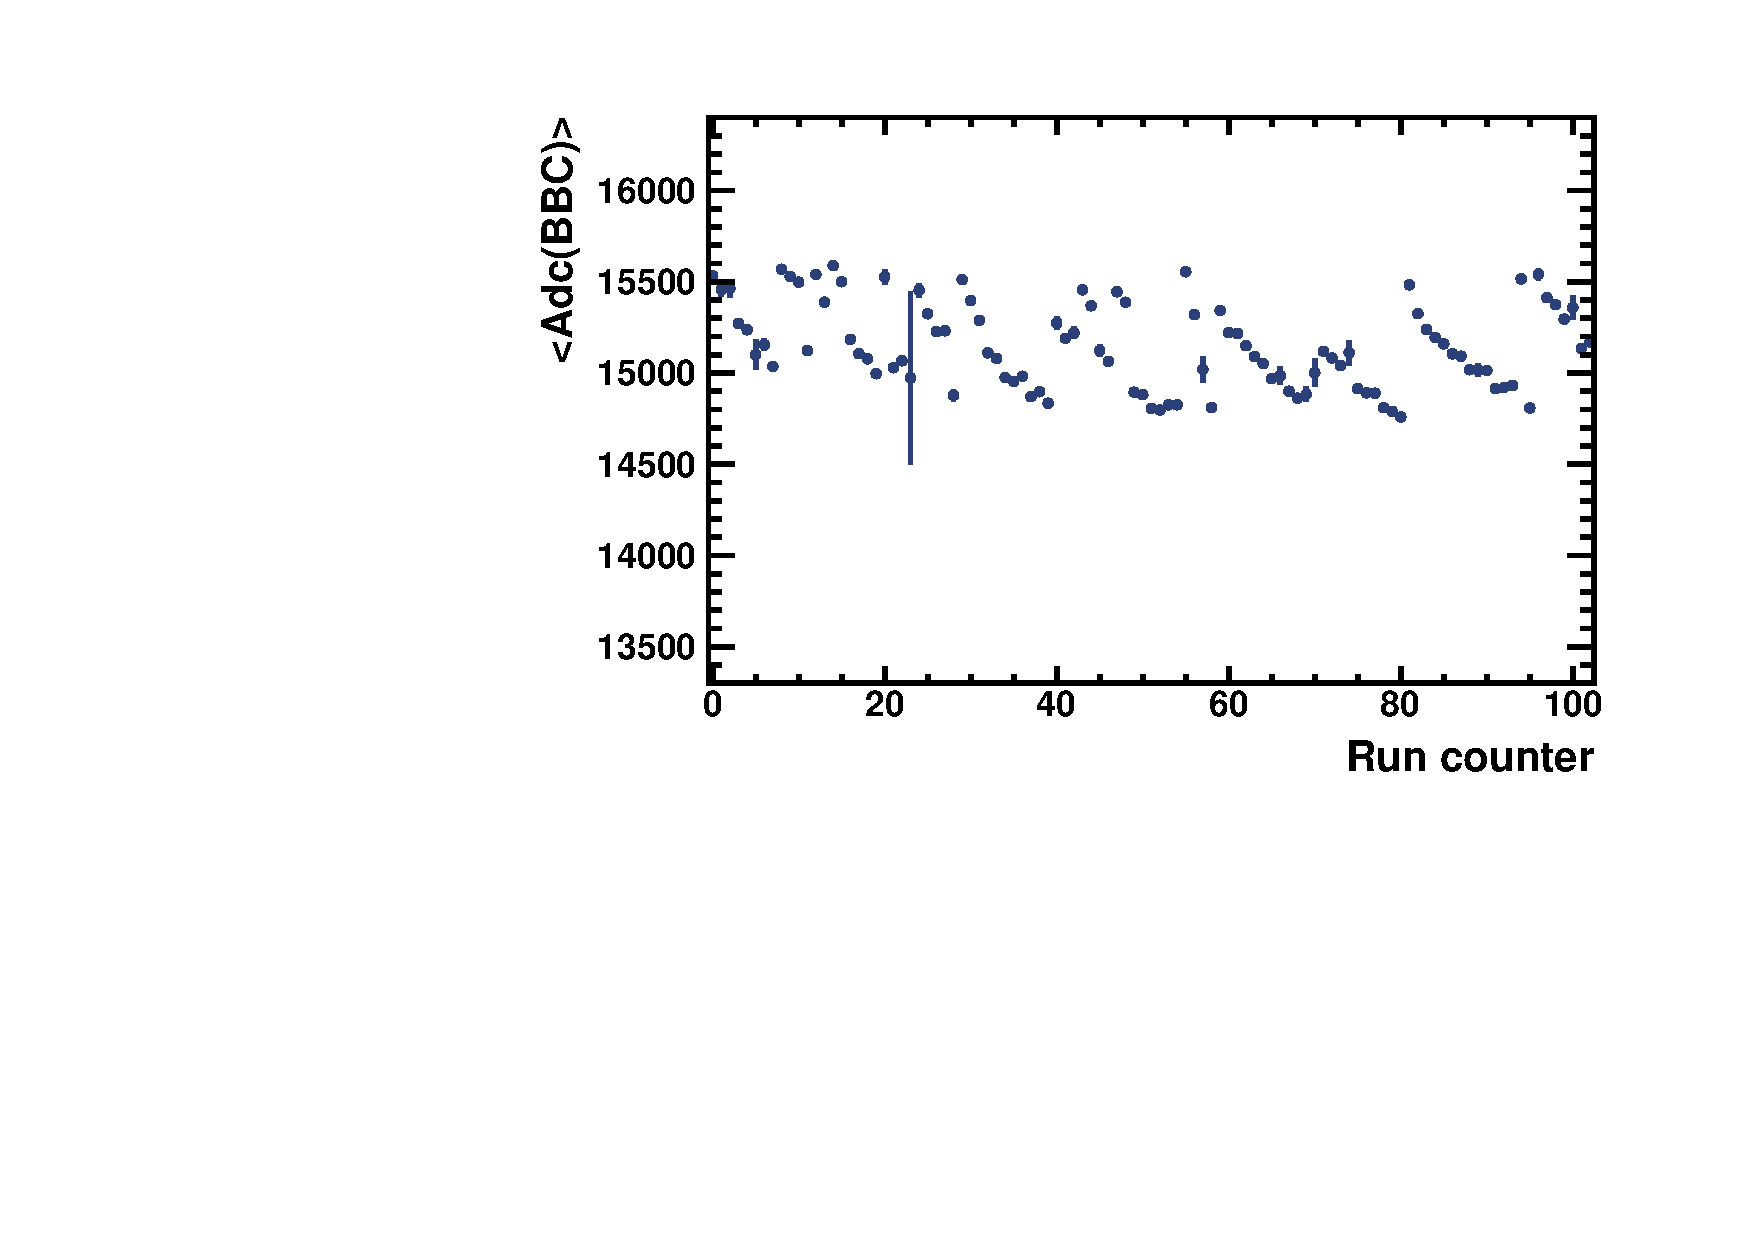
\includegraphics[width=1.\linewidth]{Figures/AdcVsRun.pdf}
        %\caption{b}
    \end{subfigure}
    \label{fig:RefMultAdcVsRun}
    \caption{Distributions of the RefMult (left) and Adc from \BBC\ (right) as a function of run.}
\end{figure}

\begin{figure}[ht]
    \begin{subfigure}{.49\textwidth}
        \centering
        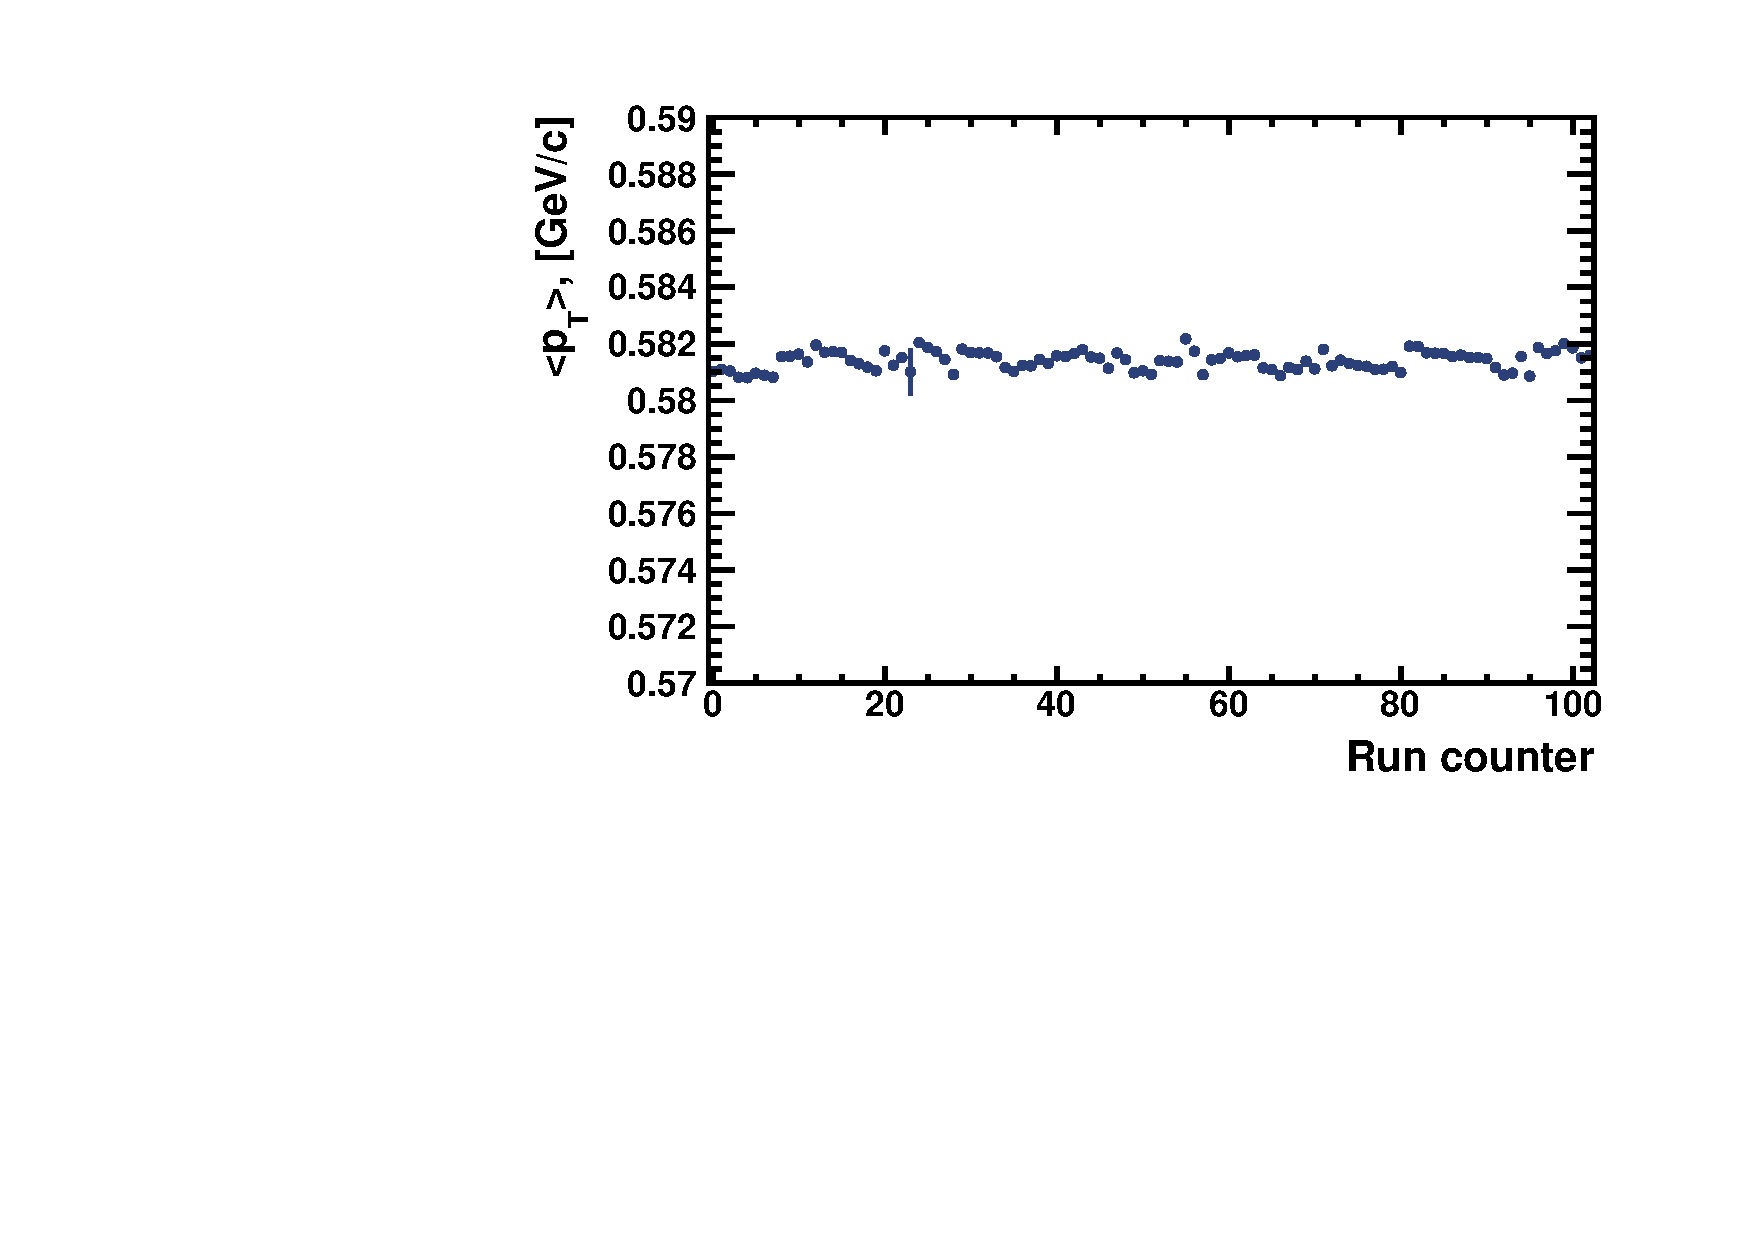
\includegraphics[width=1.\linewidth]{Figures/PtVsRun.pdf}
        %\caption{a}
    \end{subfigure}
    \begin{subfigure}{.49\textwidth}
        \centering
        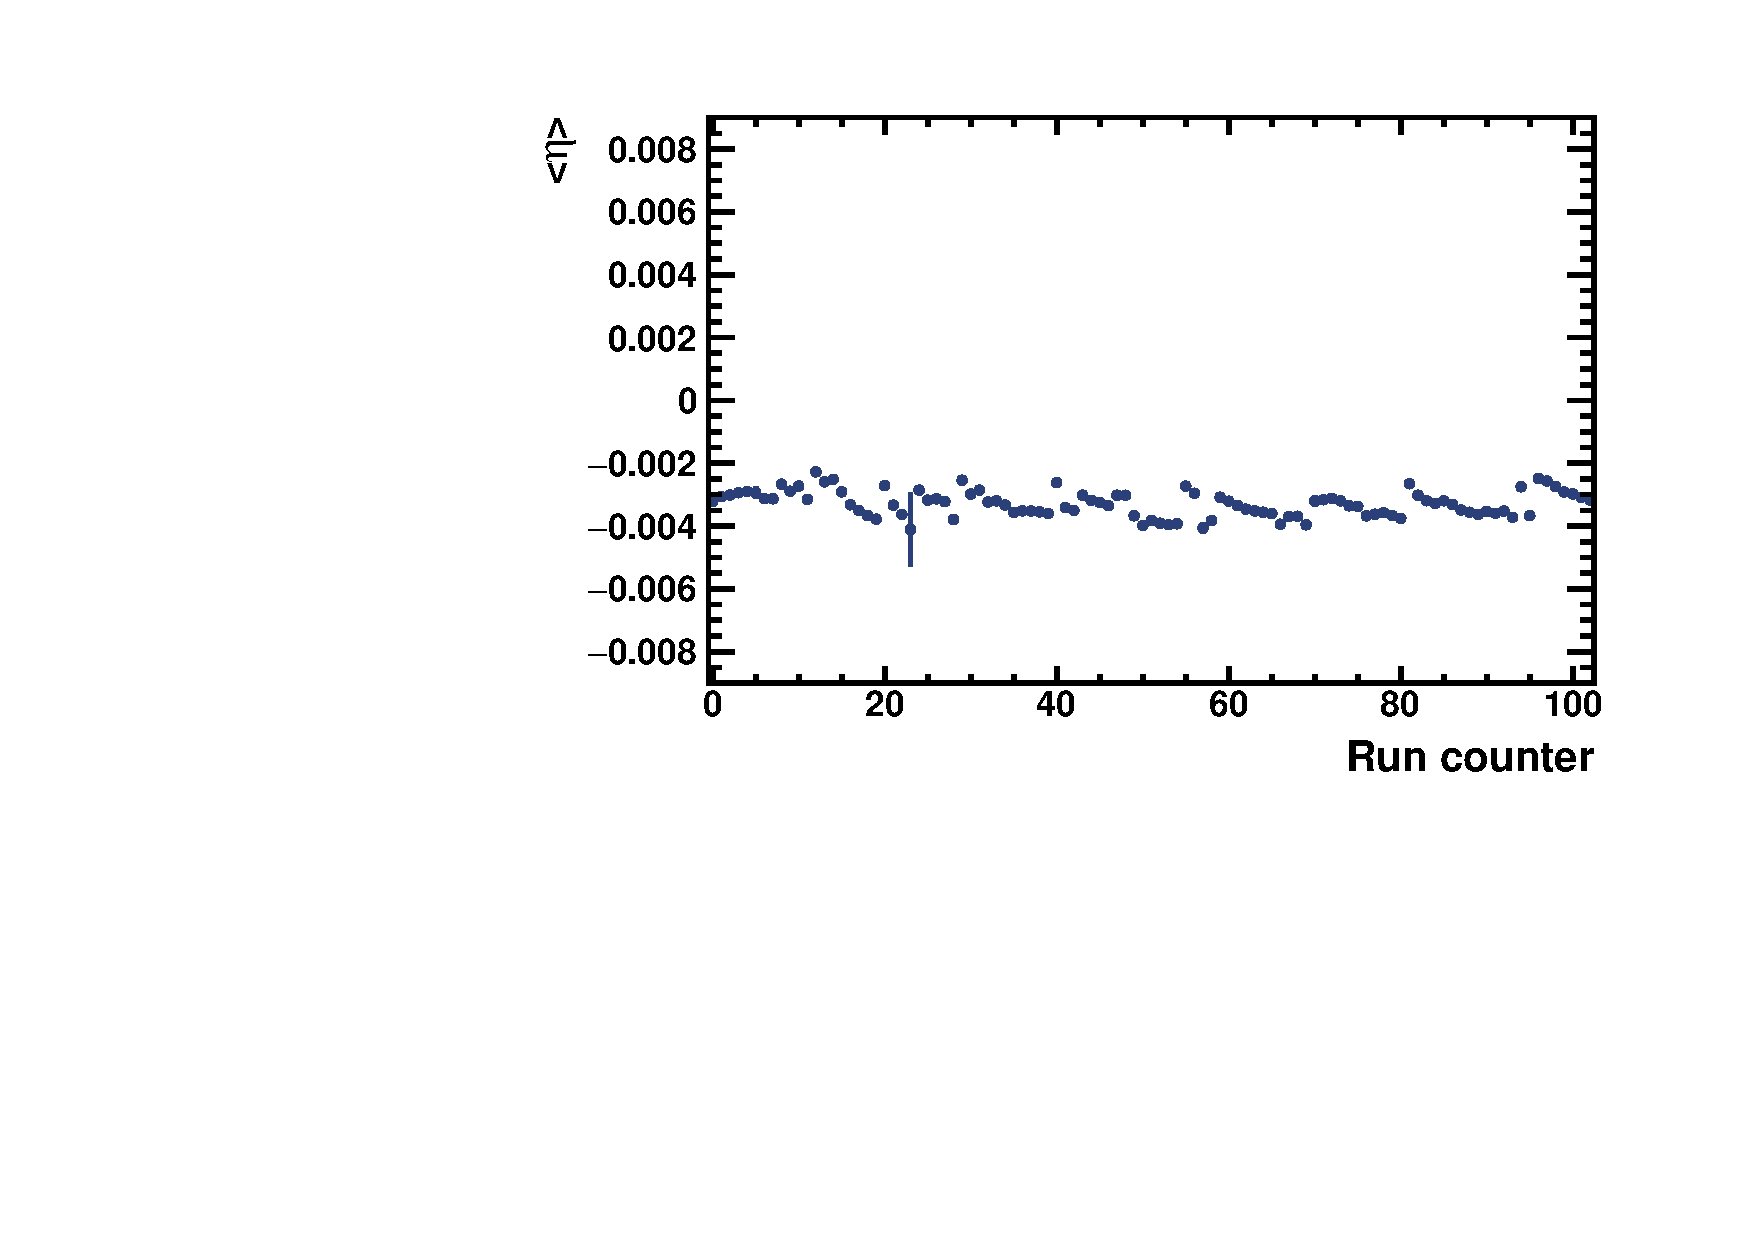
\includegraphics[width=1.\linewidth]{Figures/EtaVsRun.pdf}
        %\caption{b}
    \end{subfigure}
    \\
    \begin{subfigure}{.49\textwidth}
        \centering
        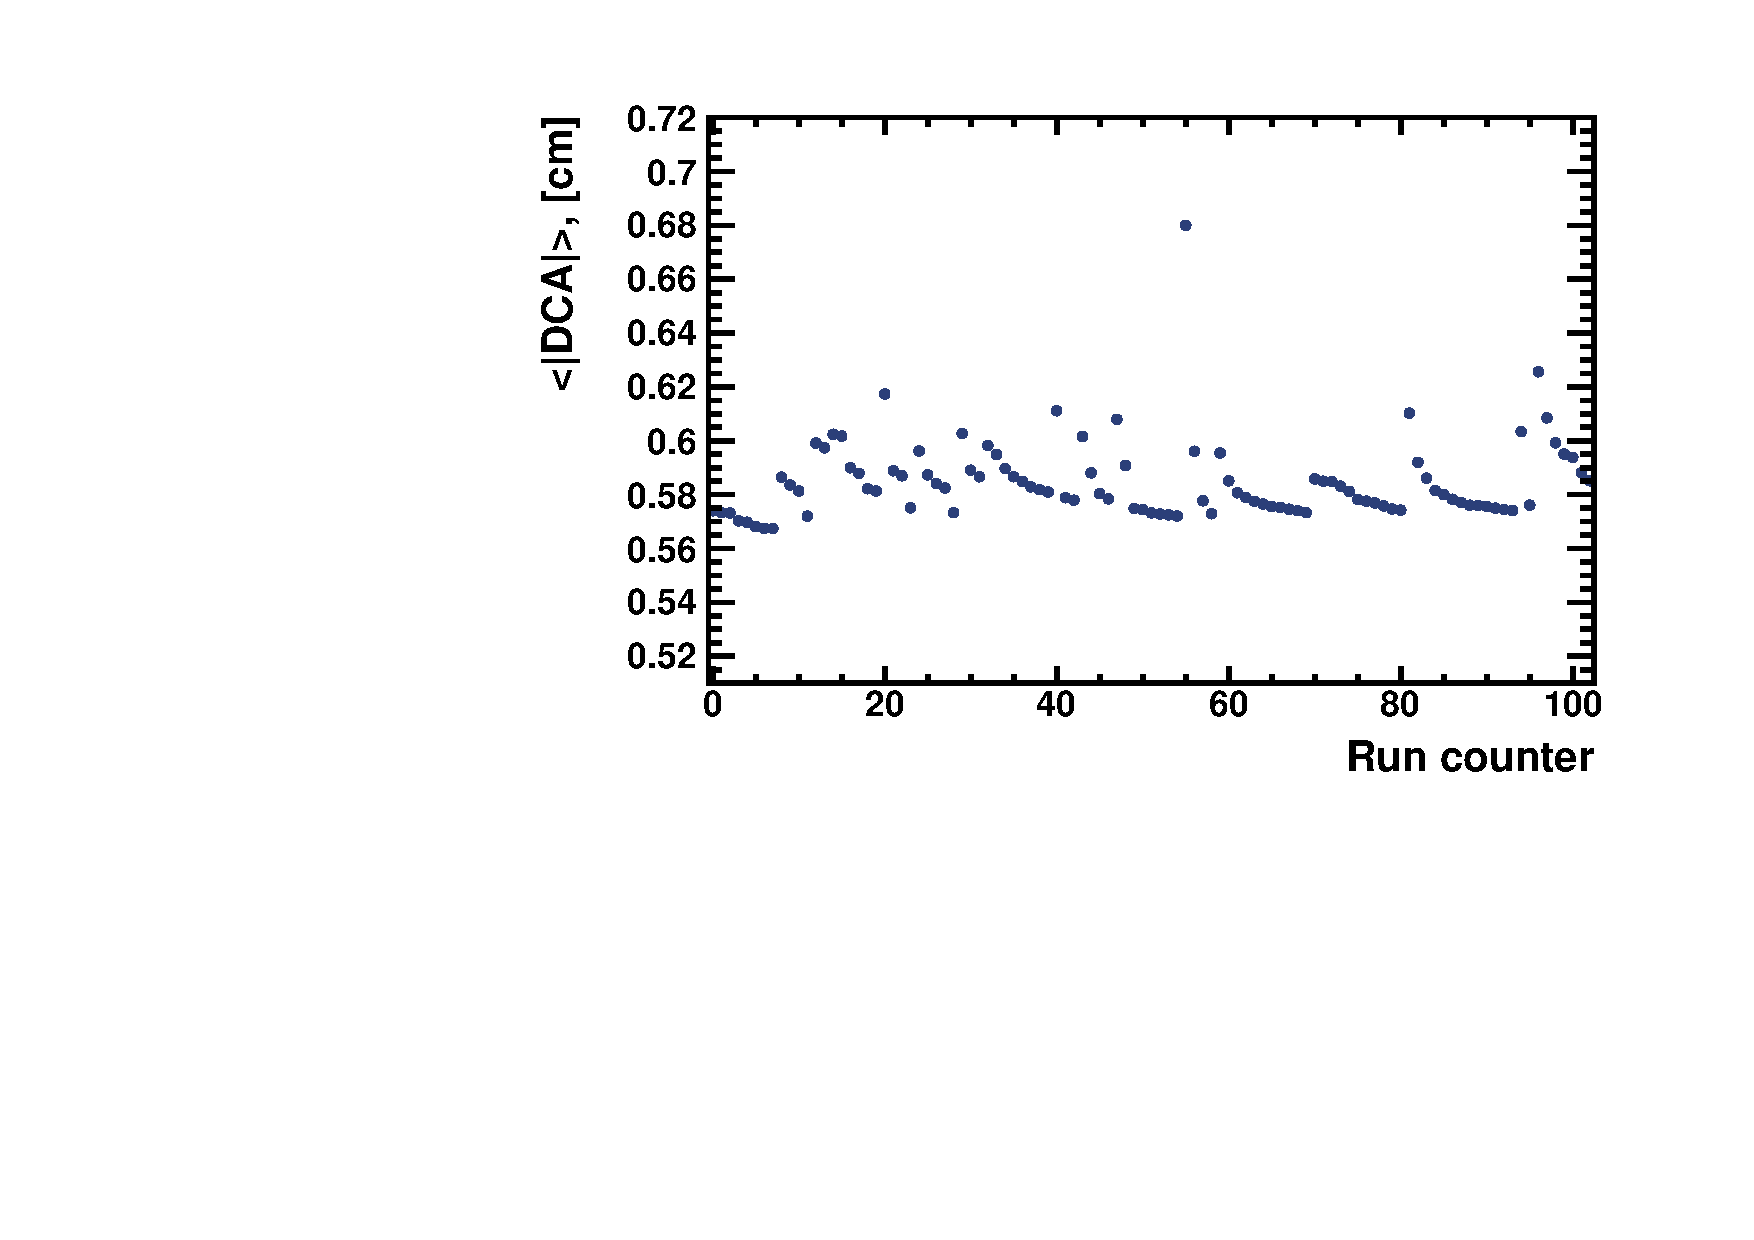
\includegraphics[width=1.\linewidth]{Figures/DCAVsRun.pdf}
        %\caption{a}
    \end{subfigure}
    \begin{subfigure}{.49\textwidth}
        \centering
        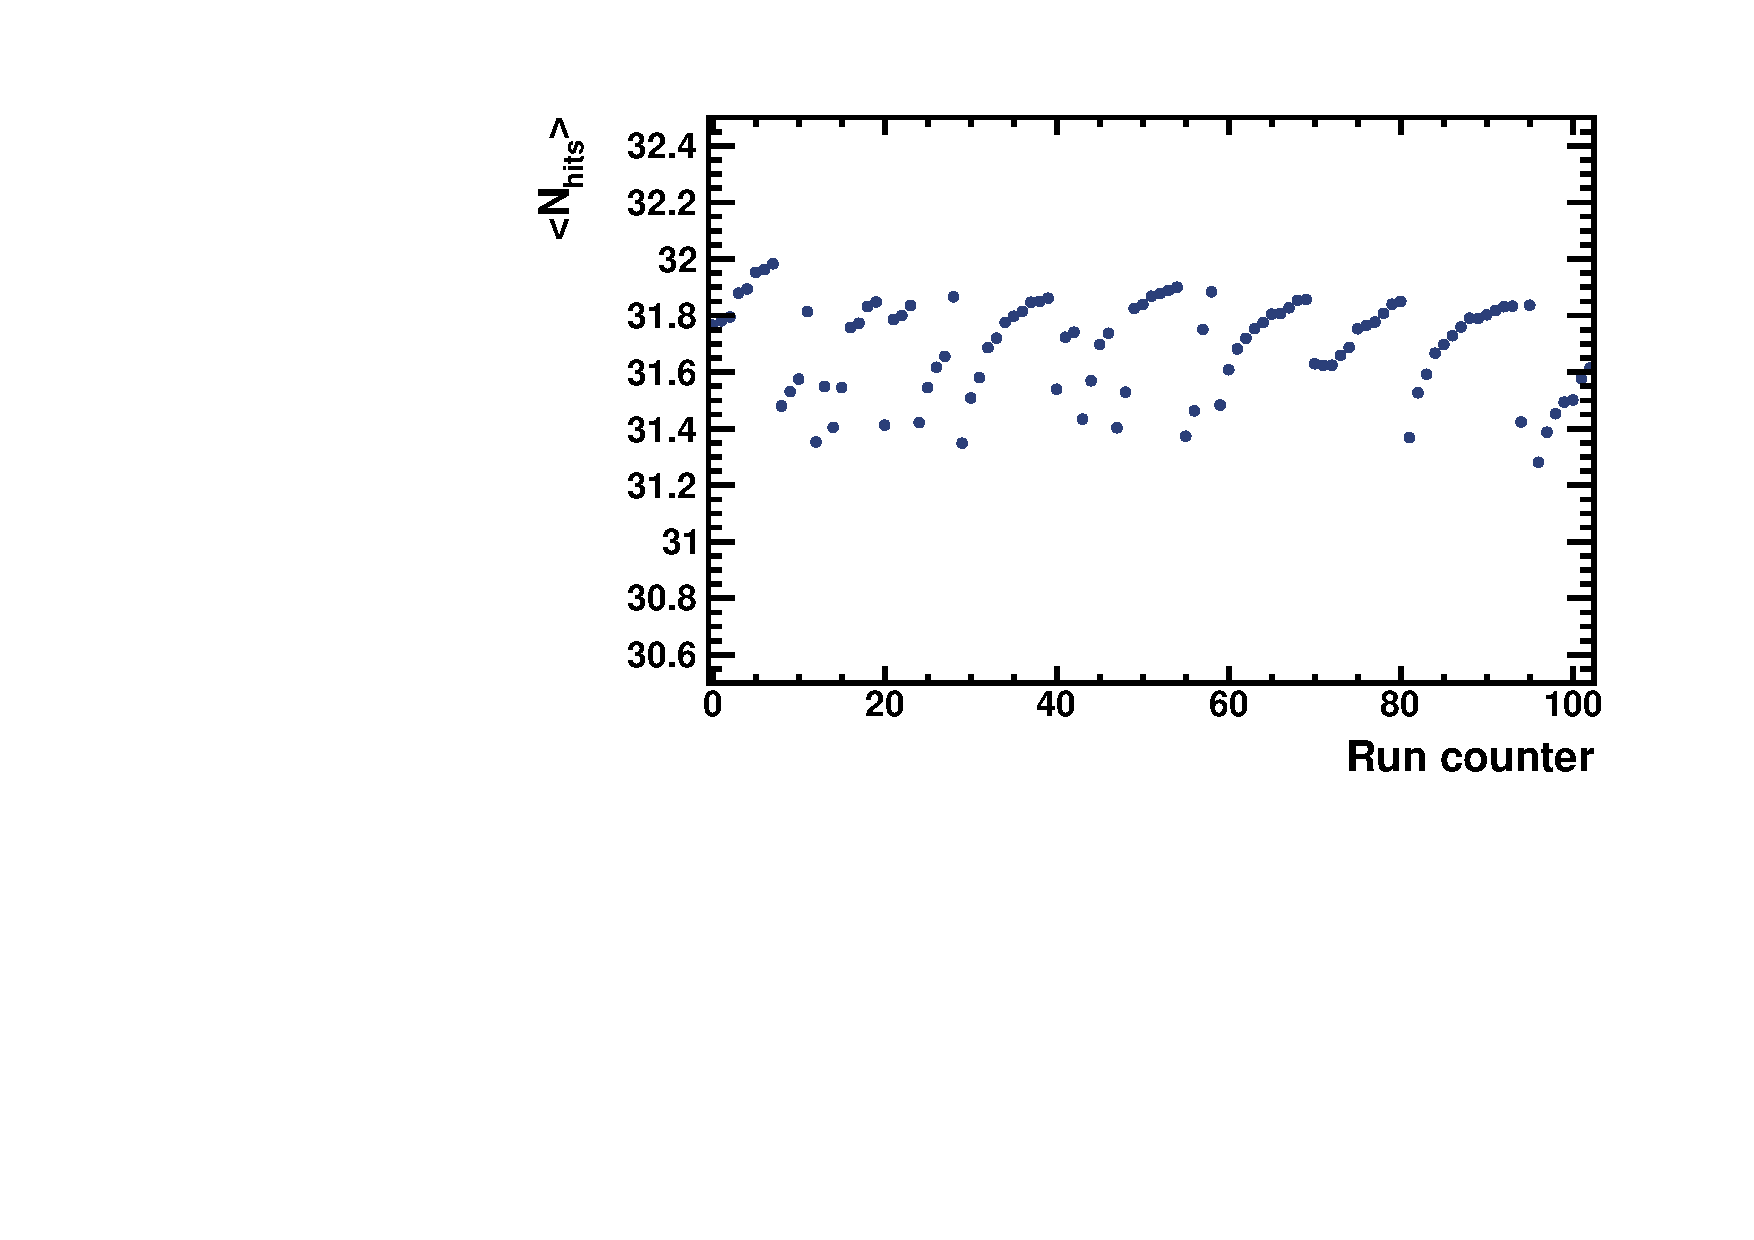
\includegraphics[width=1.\linewidth]{Figures/NhitsFitVsRun.pdf}
        %\caption{b}
    \end{subfigure}
    \label{fig:TrackVsRun}
    \caption{Distributions of the $p_{T}$ (upper left), $\eta$ (upper right), \DCA\ (bottom left) and $N_{hits}$ (bottom right) as a function of run.}
\end{figure}